\documentclass[border=4pt]{standalone}
\usepackage[T1]{fontenc}
\usepackage{helvet}
\renewcommand{\familydefault}{\sfdefault}
\usepackage{graphicx}
\usepackage{caption}
\usepackage{amsmath}
\captionsetup{font={sf,footnotesize},labelfont={sf,bf,footnotesize},justification=justified,singlelinecheck=false}
\begin{document}
\setcounter{figure}{0}
\renewcommand{\thefigure}{S\arabic{figure}}
\begin{minipage}{7.20in}
\centering
\begin{figure}[htbp]
    \centering
    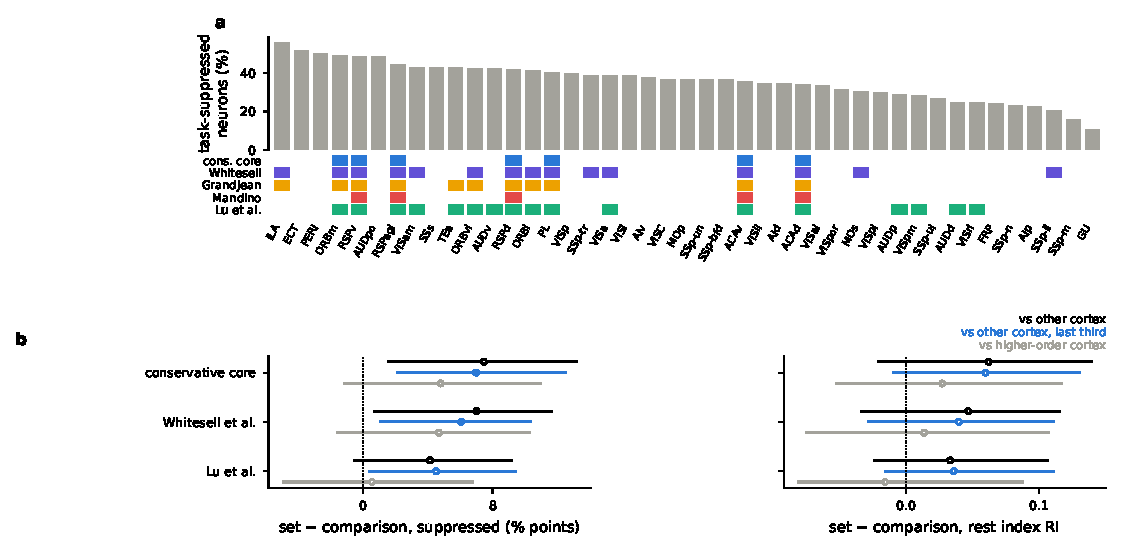
\includegraphics[width=\linewidth]{figS1_whitesell_restpref_panels.pdf}
    \caption{\textbf{a} Task-suppressed neurons per cortical region relative to the grey screen (as Fig. 3a, grey bars), with region membership in four DMN definitions underneath. Whitesell et al. (2021): cortical regions with $>$50\% of voxels in the core DMN mask of mouse rsfMRI group ICA, registered to the Allen CCFv3 (ACA, PL, ILA, ORB, RSP, VISa, VISam, SSp-tr, SSp-ll, MOs). They do not include TEa, ECT or PERI (our lateral extension), which lie in their separate lateral cortical network. \textbf{b} Each definition minus other cortex (black), the same against only the last third of trials (blue), and minus higher-order cortex only (grey): 95\% mouse-bootstrap CI; filled markers, region-permutation p $<$ 0.05. The Whitesell set is weaker than ours because it adds the task-driven SSp-tr, SSp-ll and MOs and leaves out TEa, ECT and PERI.}
    \label{fig:grey_s1}
\end{figure}
\end{minipage}
\end{document}
